\subsection{Der Aharanov-Bohn-Effekt} \marginpar{14.12.15}
(Ehrenberg-Siday 1949, (wieder entdeckt bzw mathematisch besser:)Aharanov-Bohn 1959)
	\begin{figure*} [h]
	\begin{center}
		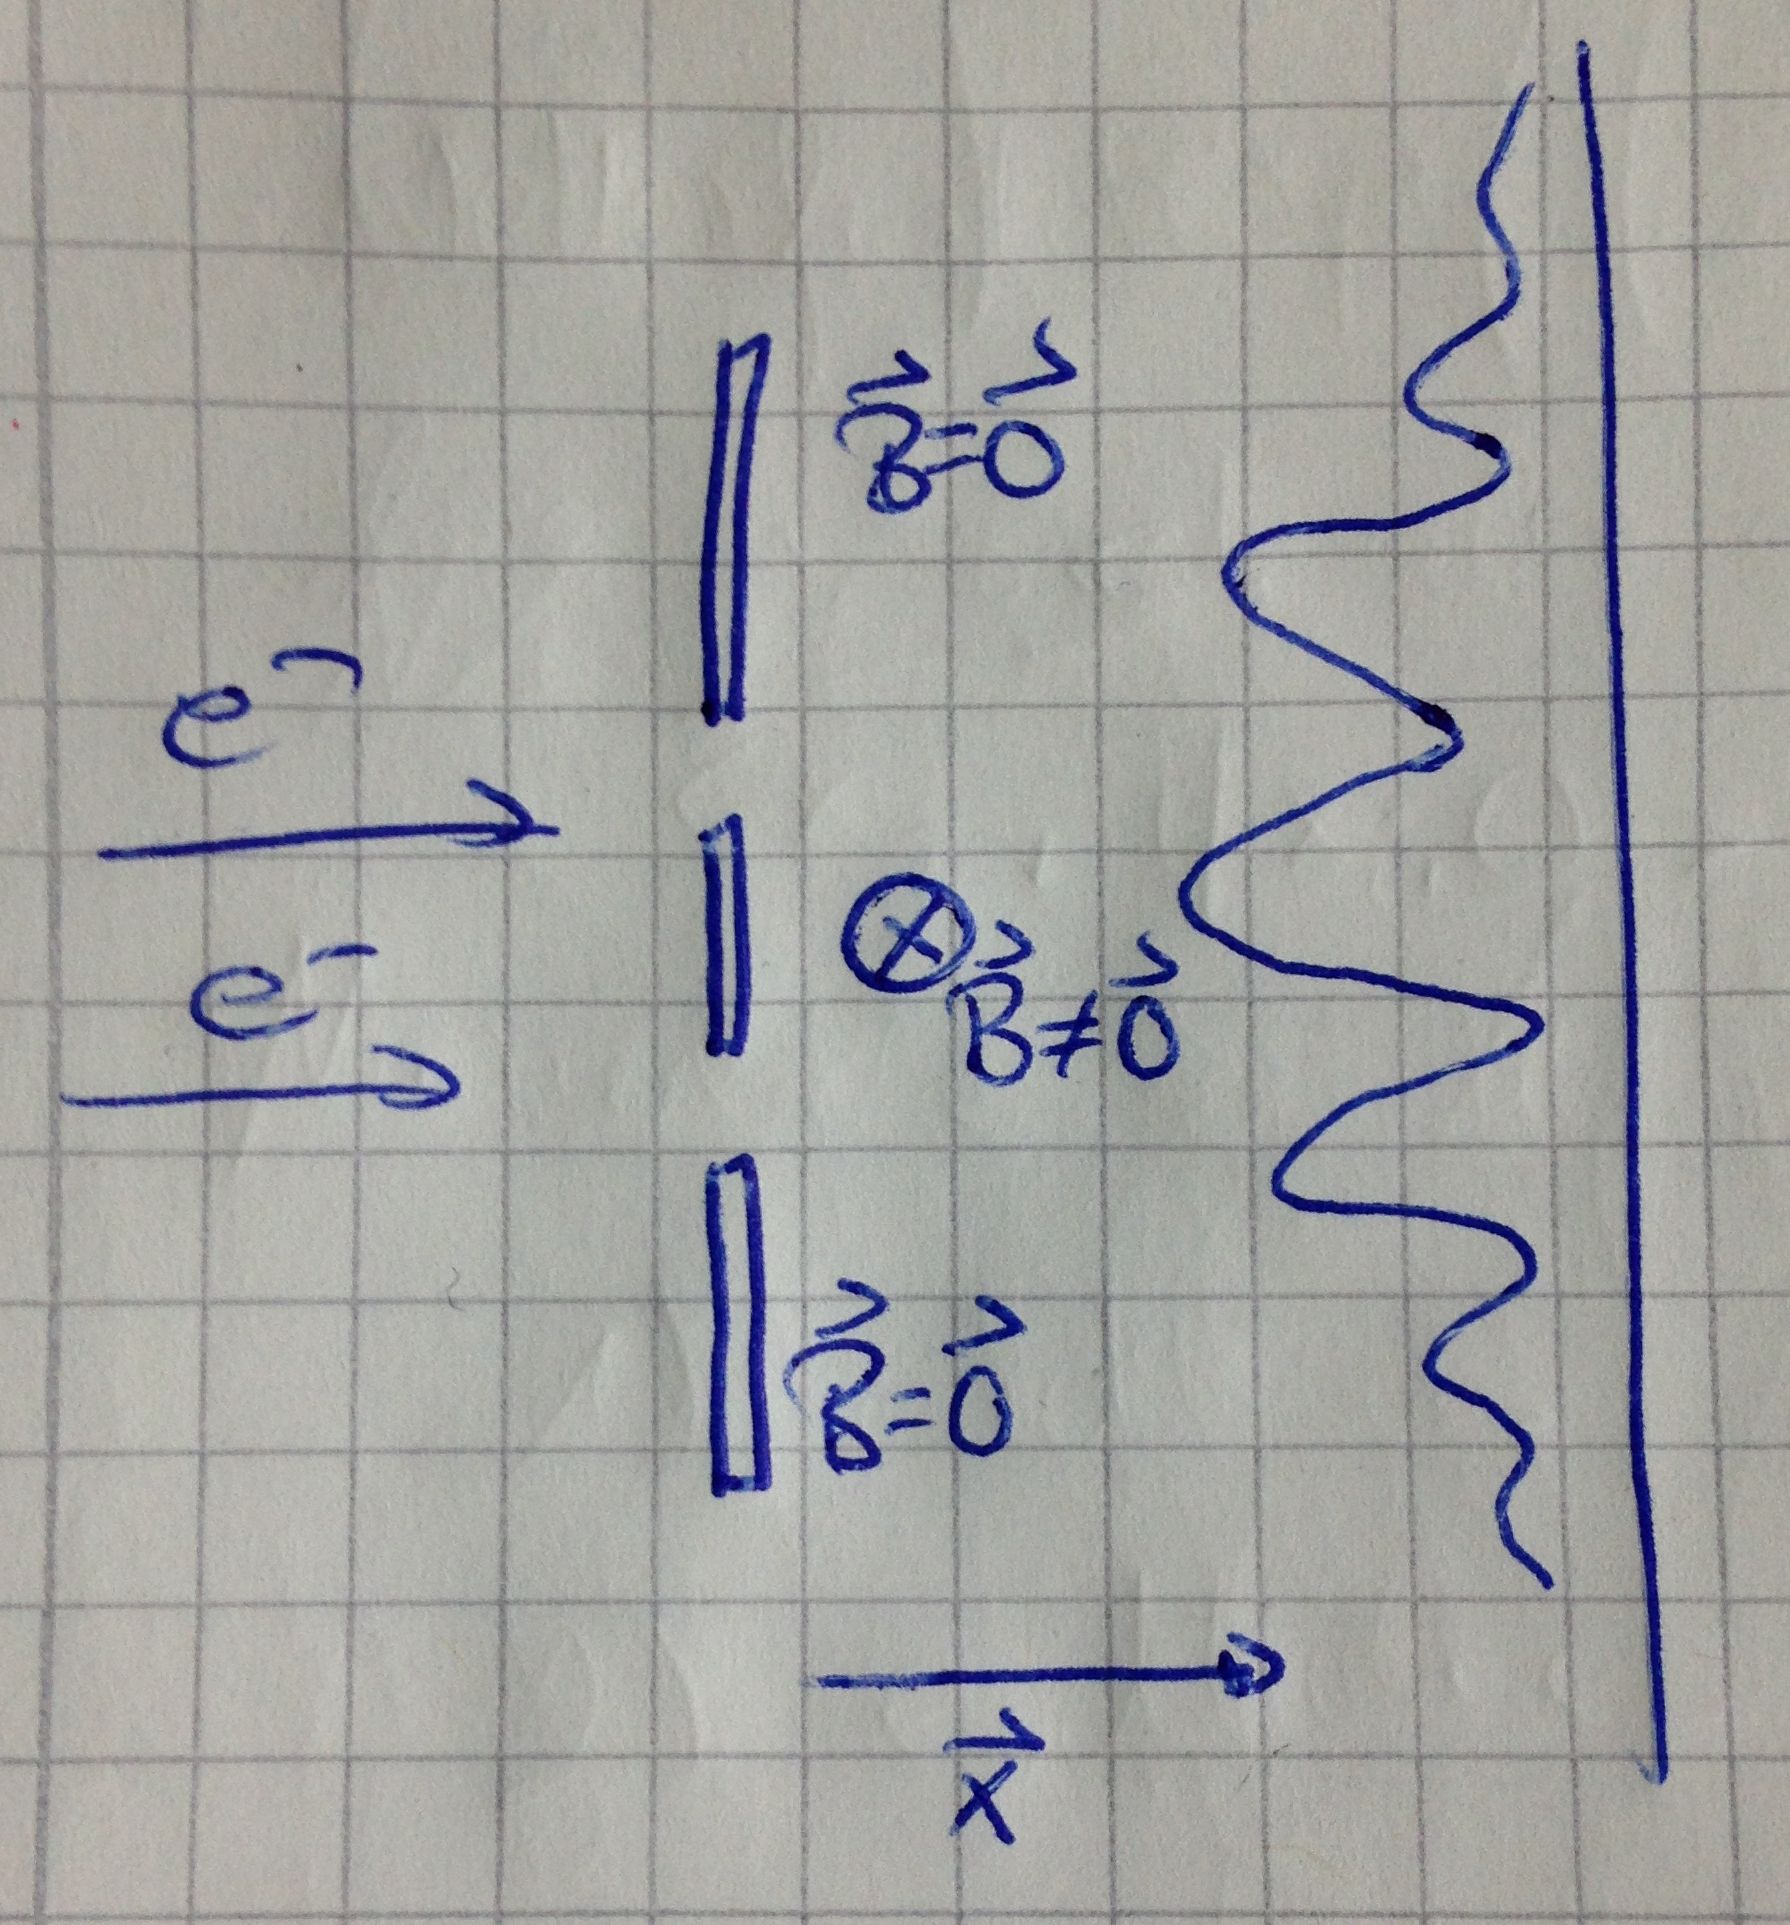
\includegraphics[width=8cm]{Aharanov-Bohn-Effekt1}
	\end{center}
	\end{figure*}
Behauptung: $\vec{B}$ beeinflusst Interferenzmuster

Klassische Physik:
	\begin{align*}
		m \ddot{\vec{r}} &= \frac{q}{c} \dot{\vec{r}} \times \vec{B} \\
		\vec{B} &= \vec{\nabla} \times \vec{A}
	\end{align*}
Beispiel:
	\begin{align*}
		\vec{A}(\vec{r}) &= \frac{\Phi m}{2\pi} \frac{(-y,x,0)}{x^2 + y^2} \\
		\int \diff x \diff y \vec{e}_z \cdot \vec{B}(x,y,z) &=
		\oint_{\partial F} \diff \vec{r} \cdot \vec{A}(\vec{r})=
		\int_{0}^{2 \pi} \diff \phi ~r_{\perp} \frac{\Phi m}{2 \pi} \frac{r_{\perp}}{r_{\perp}^2} \vec{e}_\phi \cdot \vec{e}_\phi \\
		&=\Phi_m ~\text{für jedes } r_{\perp} > 0
	\end{align*}
$\Phi_m$: Magnetisscher Fluß (durch $F$)
	\begin{align*}
		\vec{B} &= \vec{e}_z \cdot \Phi_m \delta^{(3)}(x,y) \\
		\text{Weil } \int_F \diff \vec{f} \cdot \vec{B} &= \Phi_m,&
		\text{Aber } \vec{\nabla} \times \vec{A} \text{ divergiert für } r_{\perp} \rightarrow \infty
	\end{align*}
$\vec{B} = 0$, außer bei $x=y=0$. Aber $\vec{A}(\vec{r}) \neq \vec{0}$ überall.

$\vec{A}(\vec{r})$ ist nur festgelegt bis auf eine Eichtransformation:
	\begin{align*}
		\vec{A} \mapsto \vec{A} + \vec{\nabla} \Lambda (\vec{r}(t)) 
		\Rightarrow \vec{B}(\vec{r}) \mapsto \vec{B}(\vec{r})
	\end{align*}
Lagrangefunktion:
	\begin{align*}
		L &= \frac{m}{2} \dot{\vec{r}}^2 + \frac{q}{c} \dot{\vec{r}} \cdot \vec{A}
		& \frac{\diff}{\diff t} \frac{\partial L}{\partial \dot{r}_i} - \frac{\partial L}{\partial r_i} &= 0 &
		\Rightarrow m \ddot{\vec{r}} &= \frac{q}{c} (\dot{\vec{r}} \times(\vec{\nabla} \times \vec{A})) \\
		&= L_0 + \frac{q}{c} \dot{\vec{r}} \cdot \vec{A}
	\end{align*}
	\begin{align*}
		S &= S_0 + \frac{q}{c} \int_{t_0}^{t_1} \diff t ~\dot{\vec{r}} \cdot \vec{A}(\vec{r}(t)) \\
		&= S_0 + \frac{q}{c} \int_{\vec{r}(t_0) = \vec{y}}^{\vec{r}(t_1) = \vec{x}} \diff \vec{r} \cdot \vec{A}(\vec{r}) 
	\end{align*}
$\vec{A}(\vec{r}) \neq \vec{\nabla}$ (Skalarfeld)(Problem bei $x=y=0$), deshalb wird das zweite Integral wegabhängig sein
	\begin{figure*} [h]
		\begin{center}
			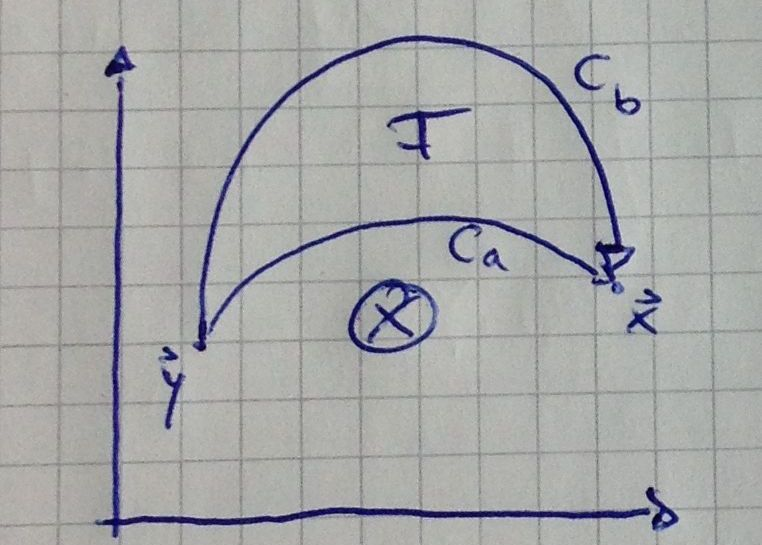
\includegraphics[width=8cm]{Aharanov-Bohn-Effekt2}
		\end{center}
	\end{figure*}
\FloatBarrier
	\begin{align*}
		\int_{c_a} \diff \vec{r} \cdot \vec{A}(\vec{r}) - \int_{c_b} \diff \vec{r} \cdot \vec{A}(\vec{r}) &=
		\oint_{c_a-c_b} \overset{Stokes}{=} 
		\int_F \diff \vec{f} (\vec{\nabla} \times \vec{A}) = \int_F \diff \vec{f} \cdot \vec{B}(\vec{r}) =0 \\
		&\Rightarrow 
		\int_{c_a} \diff \vec{r} \vec{A}(\vec{r}) = \int_{c_b} \diff \vec{r} \vec{A}(\vec{r}) =
		\alpha_1 = \int_{c^{(1)}} \diff \vec{r} \cdot \vec{A}(\vec{r})
	\end{align*}
\FloatBarrier
		\begin{figure*} [h]
		\begin{center}
			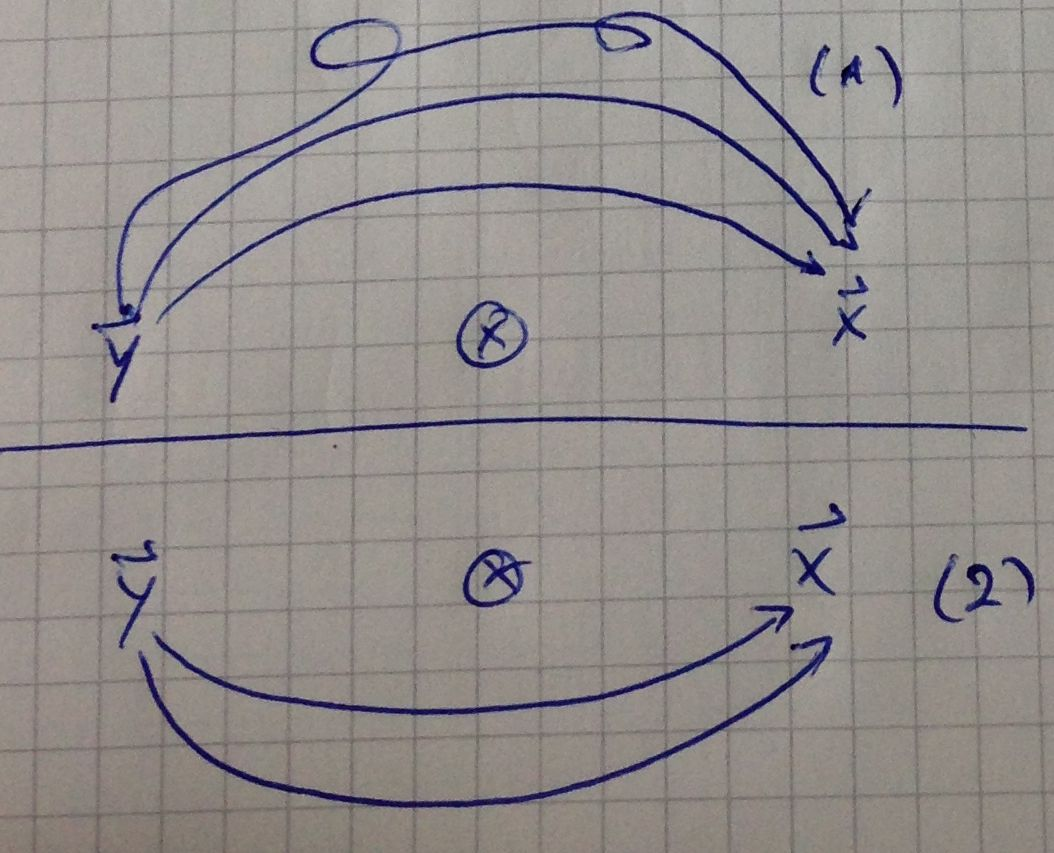
\includegraphics[width=10cm]{Aharanov-Bohn-Effekt3}
		\end{center}
		\end{figure*} 
\FloatBarrier
	\begin{align*}
		\int_{c^{(2)}} \diff \vec{r} \vec{A}(\vec{r}) = \alpha_2
	\end{align*}
\FloatBarrier
		\begin{figure*} [h]
		\begin{center}
			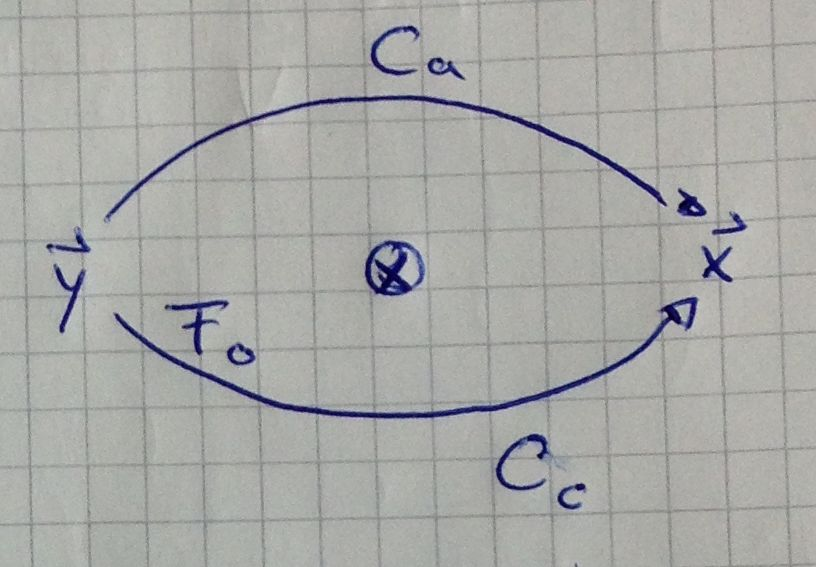
\includegraphics[width=10cm]{Aharanov-Bohn-Effekt4}
		\end{center}
		\end{figure*}
\FloatBarrier
	\begin{align*}
		\int_{c_a} \diff \vec{r} \cdot \vec{A}(\vec{r}) - \int_{c_c} \diff \vec{r} \cdot \vec{A}(\vec{r}) &=
		\int_{c^{(1)}} \diff \vec{r} \cdot \vec{A}(\vec{r}) - \int_{c^{(2)}} \diff \vec{r} \cdot \vec{A}(\vec{r}) = \alpha_1 - \alpha_2 \\
		&= \oint_{\partial F_0} \diff \vec{f} \cdot \vec{A}(\vec{r}) 
		\overset{Stokes}{=} \int_{F_0} \diff \vec{f} \cdot \vec{B}(\vec{r}) = \Phi_m
	\end{align*}
	\begin{empheq}[box=\boxed]{align*}
		\Phi_m = \alpha_1 - \alpha_2
	\end{empheq}
Übergangsamplitude
	\begin{align*}
		{}_H \braket{\vec{x}; t_1 | \vec{y}; t_0}_H &= 
		\int [\diff^3 r] e^{i \frac{S[\vec{r}(t)]}{\hbar}} \\
		&\approx \int^{(1)} [\diff^3 r] e^{i \frac{S[\vec{r}(t)]}{\hbar}} 
		+ \int^{(2)} [\diff^3 r] e^{i \frac{S[\vec{r}(t)]}{\hbar}} 
	\end{align*}
	\begin{align*}
		\int^{(1)} [\diff^3 r] e^{\frac{i}{\hbar} S} &=
		\int^{(1)} [\diff^3 r] e^{\frac{i}{\hbar} S_0} e^{\frac{i}{\hbar} \int \diff \vec{r} \frac{q}{c} \vec{A}} 
		= \int^{(1)} [\diff^3 r] e^{\frac{i}{\hbar} S_0} e^{\frac{iq}{\hbar c} \alpha_1}  
		= K_1 e^{\frac{iq}{\hbar c} \alpha_1}\\
		\int^{(2)} [\diff^3 r] e^{\frac{i}{\hbar} S} &=
		\int^{(2)} [\diff^3 r] e^{\frac{i}{\hbar} S_0} e^{\frac{i}{\hbar} \int \diff \vec{r} \frac{q}{c} \vec{A}} 
		= \int^{(2)} [\diff^3 r] e^{\frac{i}{\hbar} S_0} e^{\frac{iq}{\hbar c} \alpha_2}
		=K_2 e^{\frac{iq}{\hbar c} \alpha_2}
	\end{align*}
	\begin{align*}
		\braket{\vec{x}; t_1| \vec{y}; t_0} &= 
		K_1 e^{\frac{iq}{\hbar c} \alpha_1} + K_2 e^{\frac{iq}{\hbar c} \alpha_2} + \ldots 
		\approx e^{\frac{iq}{\hbar c} \alpha_1} (K_1 + K_2 e^{\frac{iq}{\hbar c} (\alpha_2 -\alpha_1)})
	\end{align*}
Übergangswahrscheinlichkeitsdichte:
	\begin{align*}
		|\braket{\vec{x}; t_1 | \vec{y} , t_0}|^2 &=
		| K_1 + K_2 e^{-\frac{iq}{\hbar c} \Phi_m}|^2
	\end{align*}
hängt ab von magnetischem Fluss, obwohl Pfade (fast) nie durch Region mit $\vec{B}\neq \vec{0}$ laufen.

Korrekte Lösung:
	\begin{align*}
		|\braket{\vec{x}; t_1 | \vec{y} , t_0}|^2 &=
		\left|
			\sum_{n\in\mathds{Z}} K_{n} e^{in \frac{q}{\hbar c} \Phi_m}
		\right|^2
	\end{align*}
$n$ ist Windungszahl.
	\begin{align*}
		\Phi_m &= \frac{\hbar c}{q} 2\pi \cdot \ell ,& \ell&\in \mathds{Z} \\
	\end{align*}
$\Rightarrow$ Magnetfeld hat keinen Einfluss.

Ansonsten beeinflusst $\vec{B}$ das Interferenzmuster. 
\\
NB: Flussquantisierung in Supraleitern (London 1948)
\\ \\
Aufgabe 9:

Eichtransformation $\Lambda (\vec{r}, t)$
	\begin{align*}
		\vec{A} (\vec{r}, t) &\mapsto \vec{A} (\vec{r}, t) + \vec{\nabla} \Lambda \\
		\Phi (\vec{r}, t) &\mapsto \Phi (\vec{r}, t) + \frac{1}{c} \frac{\partial \Lambda}{\partial t} \\
		\psi (\vec{r}, t) &\mapsto \exp \left(i \frac{q}{\hbar c} \Lambda (\vec{r}, t)\right)
		\psi (\vec{r}, t)
	\end{align*}
damit Schrödingergleichung für Teilchen mit Ladung $q$ eichunabhängig ist.
$\Rightarrow$ Kann Interferenzeffekte beeinflussen.

Kovariante Ableitung:
	\begin{align*}
		\vec{D} &= \vec{\nabla} - i\frac{q}{\hbar c} \vec{A} (\vec{r},t) \\
		\vec{j} &= \frac{\hbar}{2 i m} \left(
			\psi^* \vec{D} \psi + \psi \vec{D} \psi^*
		\right),&
		\vec{\nabla} \vec{j} + \frac{\partial \rho}{\partial t} &= 0
	\end{align*}

